\chapter{Transienten Simulation}
Ziel dieser Simulation soll es sein, das zeitliche Temperaturverhalten innerhalb der Matrix zu ermitteln. Die Informationen zu diesem verhalten sind notwendig um Mausbewegungen zu simulieren. folgende Unterkapitel sollen die Ergebnisse Darstellen.
	\section{Widerstandssimulation}
	Um einen ersten Eindruck zu erhalten, wurden ein 3 x 3 Pixel Rechteck 30 s lang mit 50 mW erw�rmt und weitere 40 s ohne Leistungserzeugung simuliert. dadurch ergab sich folgender Temperaturverlauf:
	
	\begin{center}
		\begin{minipage}[!ht]{0.6\textwidth}
			\captionsetup{type=figure}
			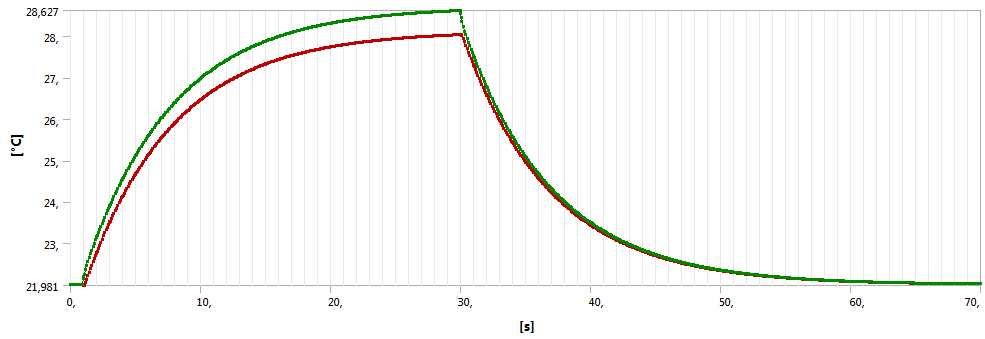
\includegraphics[width=1\linewidth]{bilder/Aufwaermeverlauf}
			\caption{Aufw�rm- und Abk�hlezyklus}
			\label{fig:Aufwaermeverlauf}
		\end{minipage}
	\end{center}	
	Zu beobachten ist, dass erst nach 30 Sekunden ein statisches verhalten erkennbar ist. somit kann bei einer Belastungszeit von einer Sekunde kein Maximalwert erreicht werden. um das dynamische verhalten zu verbessern wird die Bewegungssimulation mit 150 mW durchgef�hrt.
	
	Um nun die Bewegungseinfluss zu simulieren wurden das oben benannte Pixelquadrat Simuliert. Dabei zeigte sich, das die Platine Die Quelle �berstrahlt. Daraufhin wurde eine weitere Simulation gestartet, bei der nur ein Pixel �ber das Feld wandernd angesteuert wird. Jedoch konnte diese Simulation nicht Fehlerfrei abgeschlossen werden.